% Options for packages loaded elsewhere
\PassOptionsToPackage{unicode}{hyperref}
\PassOptionsToPackage{hyphens}{url}
%
\documentclass[
  11pt,
  ignorenonframetext,
]{beamer}
\usepackage{pgfpages}
\setbeamertemplate{caption}[numbered]
\setbeamertemplate{caption label separator}{: }
\setbeamercolor{caption name}{fg=normal text.fg}
\beamertemplatenavigationsymbolsempty
% Prevent slide breaks in the middle of a paragraph
\widowpenalties 1 10000
\raggedbottom
\setbeamertemplate{part page}{
  \centering
  \begin{beamercolorbox}[sep=16pt,center]{part title}
    \usebeamerfont{part title}\insertpart\par
  \end{beamercolorbox}
}
\setbeamertemplate{section page}{
  \centering
  \begin{beamercolorbox}[sep=12pt,center]{part title}
    \usebeamerfont{section title}\insertsection\par
  \end{beamercolorbox}
}
\setbeamertemplate{subsection page}{
  \centering
  \begin{beamercolorbox}[sep=8pt,center]{part title}
    \usebeamerfont{subsection title}\insertsubsection\par
  \end{beamercolorbox}
}
\AtBeginPart{
  \frame{\partpage}
}
\AtBeginSection{
  \ifbibliography
  \else
    \frame{\sectionpage}
  \fi
}
\AtBeginSubsection{
  \frame{\subsectionpage}
}
\usepackage{amsmath,amssymb}
\usepackage{lmodern}
\usepackage{iftex}
\ifPDFTeX
  \usepackage[T1]{fontenc}
  \usepackage[utf8]{inputenc}
  \usepackage{textcomp} % provide euro and other symbols
\else % if luatex or xetex
  \usepackage{unicode-math}
  \defaultfontfeatures{Scale=MatchLowercase}
  \defaultfontfeatures[\rmfamily]{Ligatures=TeX,Scale=1}
\fi
\usetheme[]{metropolis}
% Use upquote if available, for straight quotes in verbatim environments
\IfFileExists{upquote.sty}{\usepackage{upquote}}{}
\IfFileExists{microtype.sty}{% use microtype if available
  \usepackage[]{microtype}
  \UseMicrotypeSet[protrusion]{basicmath} % disable protrusion for tt fonts
}{}
\makeatletter
\@ifundefined{KOMAClassName}{% if non-KOMA class
  \IfFileExists{parskip.sty}{%
    \usepackage{parskip}
  }{% else
    \setlength{\parindent}{0pt}
    \setlength{\parskip}{6pt plus 2pt minus 1pt}}
}{% if KOMA class
  \KOMAoptions{parskip=half}}
\makeatother
\usepackage{xcolor}
\newif\ifbibliography
\usepackage{graphicx}
\makeatletter
\def\maxwidth{\ifdim\Gin@nat@width>\linewidth\linewidth\else\Gin@nat@width\fi}
\def\maxheight{\ifdim\Gin@nat@height>\textheight\textheight\else\Gin@nat@height\fi}
\makeatother
% Scale images if necessary, so that they will not overflow the page
% margins by default, and it is still possible to overwrite the defaults
% using explicit options in \includegraphics[width, height, ...]{}
\setkeys{Gin}{width=\maxwidth,height=\maxheight,keepaspectratio}
% Set default figure placement to htbp
\makeatletter
\def\fps@figure{htbp}
\makeatother
\setlength{\emergencystretch}{3em} % prevent overfull lines
\providecommand{\tightlist}{%
  \setlength{\itemsep}{0pt}\setlength{\parskip}{0pt}}
\setcounter{secnumdepth}{-\maxdimen} % remove section numbering
\ifLuaTeX
  \usepackage{selnolig}  % disable illegal ligatures
\fi
\IfFileExists{bookmark.sty}{\usepackage{bookmark}}{\usepackage{hyperref}}
\IfFileExists{xurl.sty}{\usepackage{xurl}}{} % add URL line breaks if available
\urlstyle{same} % disable monospaced font for URLs
\hypersetup{
  pdftitle={Análisis de presencias con procesos de puntos},
  pdfauthor={Gerardo Martín},
  hidelinks,
  pdfcreator={LaTeX via pandoc}}

\title{Análisis de presencias con procesos de puntos}
\subtitle{Particularidades}
\author{Gerardo Martín}
\date{2022-06-29}

\begin{document}
\frame{\titlepage}

\hypertarget{la-variable-de-respuesta}{%
\section{La variable de respuesta}\label{la-variable-de-respuesta}}

\begin{frame}{Regresión lineal}
\protect\hypertarget{regresiuxf3n-lineal}{}
\begin{itemize}
\item
  \(W\) son mediciones de peso en Kg
\item
  Modelo lineal:
\end{itemize}

\[W = \alpha + \beta Edad + \beta_{Sexo}\]

\begin{itemize}
\tightlist
\item
  Modelo predice peso en Kg
\end{itemize}
\end{frame}

\begin{frame}{Modelos de nicho y distribución}
\protect\hypertarget{modelos-de-nicho-y-distribuciuxf3n}{}
\begin{itemize}
\item
  Mediciones: coordenadas de presencia
\item
  ¿Qué unidades produce el modelo estadístico?
\end{itemize}
\end{frame}

\begin{frame}{Modelos de nichos y distribución}
\protect\hypertarget{modelos-de-nichos-y-distribuciuxf3n}{}
\begin{itemize}
\item
  Modelación correlativa

  \begin{itemize}
  \item
    Desconexión relativa entre análisis y predicción
  \item
    Confuso poner en perspectiva las unidades de predicción
  \end{itemize}
\item
  Procesos de puntos resuelven la desconexión

  \begin{itemize}
  \tightlist
  \item
    Datos: Puntos en Área de estudio dividida en unidades
  \end{itemize}
\end{itemize}
\end{frame}

\hypertarget{intensidad}{%
\section{Intensidad}\label{intensidad}}

\begin{frame}{Intensidad de puntos}
\protect\hypertarget{intensidad-de-puntos}{}
\begin{center}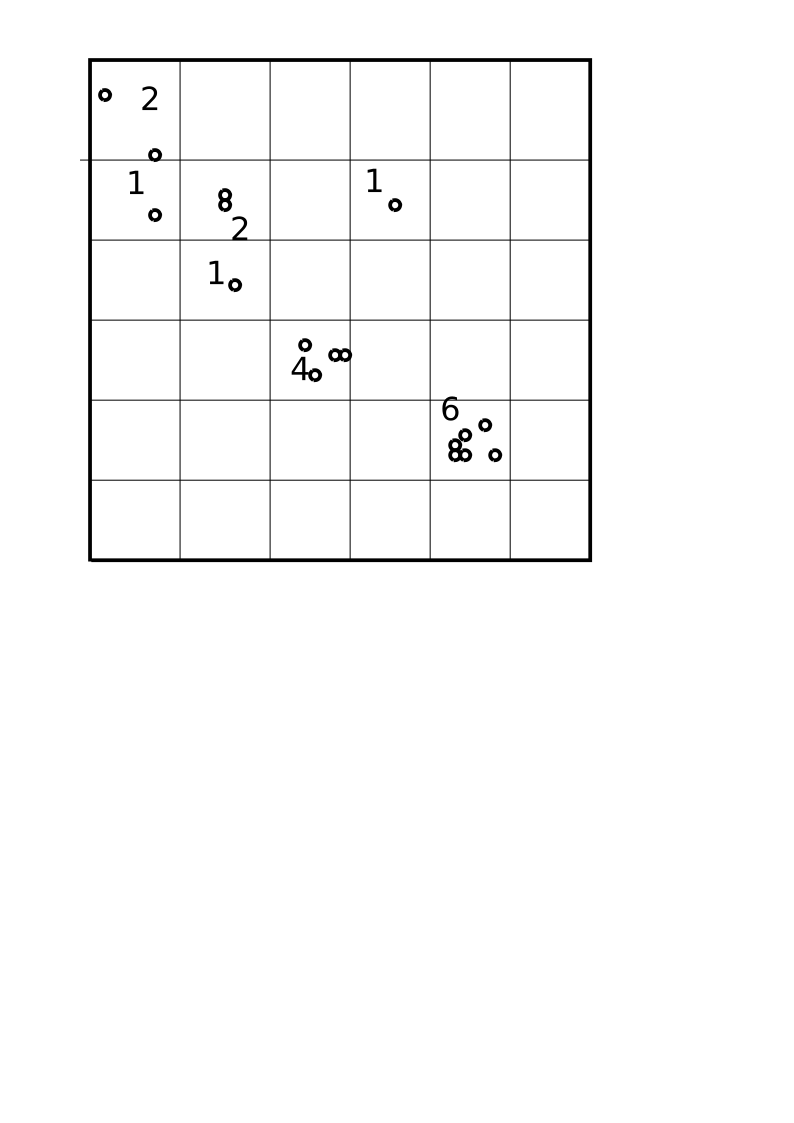
\includegraphics{Figuras/Intensidad-1} \end{center}
\end{frame}

\begin{frame}{Intensidad de puntos}
\protect\hypertarget{intensidad-de-puntos-1}{}
\begin{itemize}
\tightlist
\item
  Variable de respuesta en procesos de puntos
\end{itemize}

\[\lambda(x) = y\] - \(\lambda=\) Número promedio de puntos/unidad
espacial (píxel)
\end{frame}

\begin{frame}{Intensidad de puntos}
\protect\hypertarget{intensidad-de-puntos-2}{}
Intensidad promedio:

\begin{itemize}
\tightlist
\item
  \(\bar{\lambda} = \frac{2+2+1+1+1+4+6}{36} = \frac{17}{36}=0.47\)
\end{itemize}

Denominador es el número de unidades espaciales
\end{frame}

\begin{frame}{Intensidad de puntos}
\protect\hypertarget{intensidad-de-puntos-3}{}
\begin{figure}

{\centering 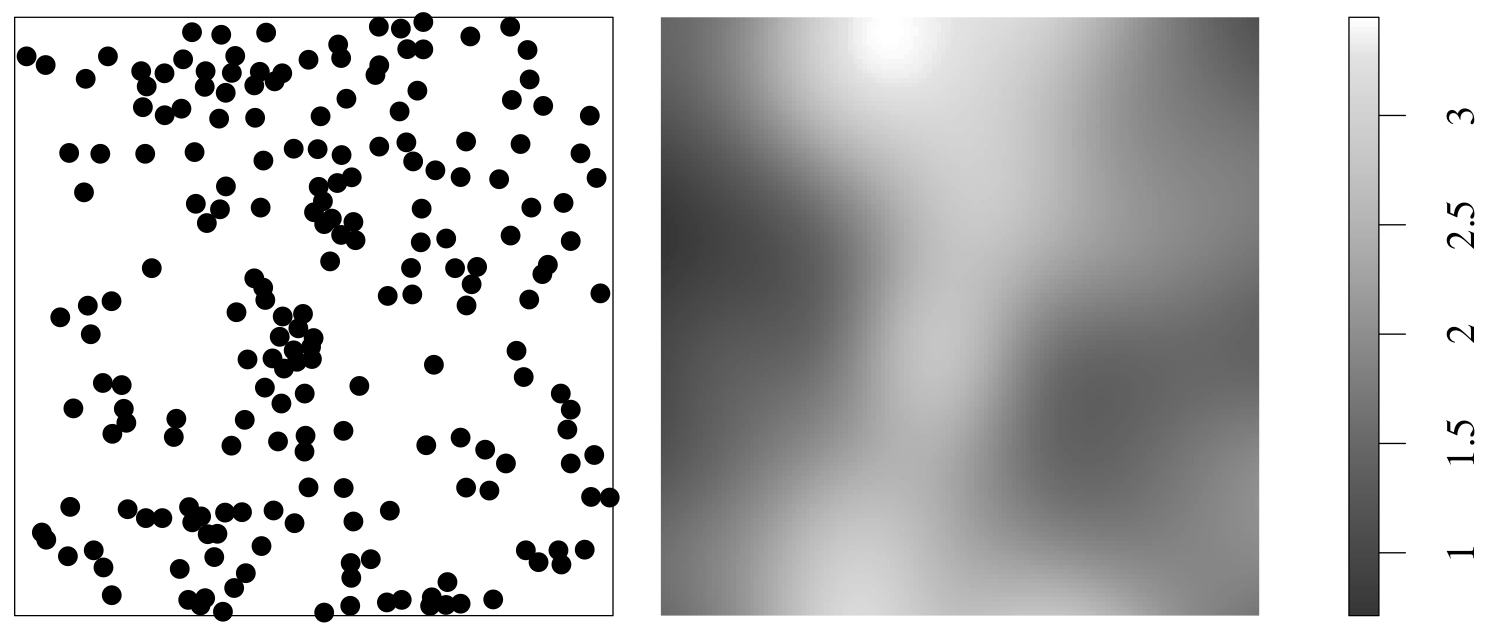
\includegraphics{Figuras/Intensidad} 

}

\caption{Ejemplo de modelo Poisson de un patrón de puntos (Baddeley et al. 2016).}\label{fig:unnamed-chunk-1}
\end{figure}
\end{frame}

\hypertarget{supuestos}{%
\section{Supuestos}\label{supuestos}}

\begin{frame}{¿Qué son los supuestos?}
\protect\hypertarget{quuxe9-son-los-supuestos}{}
\begin{itemize}
\tightlist
\item
  Postulados, premisas, cosas/hechos que se dan por sentados
\end{itemize}

\emph{Todos hacemos suposiciones y casi todas estan mal} (Einstein)

\begin{itemize}
\tightlist
\item
  Identificar bajo qué condiciones podemos estar equivocadxs
\end{itemize}
\end{frame}

\begin{frame}{Tipos de supuestos}
\protect\hypertarget{tipos-de-supuestos}{}
\textbf{Estadísticos} - Supuestos \(\rightarrow\) Errores potenciales
\(\rightarrow\) Soluciones potenciales

\textbf{Biológicos} - Supuestos estadísticos \(\rightarrow\) Problema de
estudio \(\rightarrow\) Interpretaciones
\end{frame}

\begin{frame}{Supuestos estadísticos}
\protect\hypertarget{supuestos-estaduxedsticos}{}
\begin{itemize}
\item
  Variable analizada / Modelo estadístico
\item
  Significado de los resultados
\item
  MPPs \(\rightarrow\) diferentes supuestos estadísticos

  \begin{itemize}
  \tightlist
  \item
    Distribución estadística de presencias
  \item
    Independencia
  \item
    Sesgo observacional
  \end{itemize}
\end{itemize}
\end{frame}

\begin{frame}{Supuestos estadísticos - Ejemplos}
\protect\hypertarget{supuestos-estaduxedsticos---ejemplos}{}
Media aritmética

\begin{itemize}
\tightlist
\item
  Valor más probable en distribución normal
\end{itemize}

\begin{center}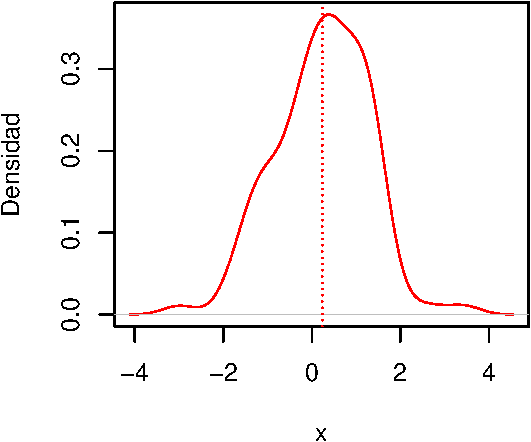
\includegraphics{Particularidades_files/figure-beamer/unnamed-chunk-2-1} \end{center}
\end{frame}

\begin{frame}{Supuestos estadísticos - Ejemplos}
\protect\hypertarget{supuestos-estaduxedsticos---ejemplos-1}{}
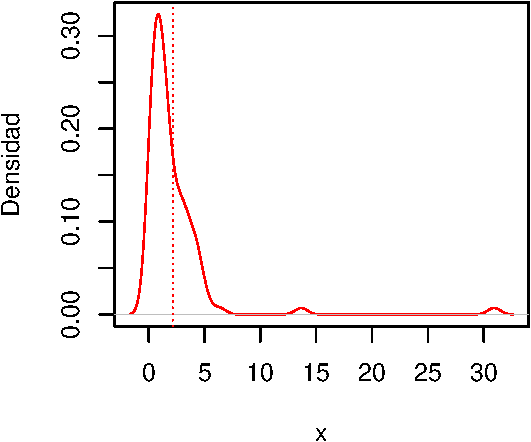
\includegraphics{Particularidades_files/figure-beamer/unnamed-chunk-3-1}
\end{frame}

\begin{frame}{Supuestos de MPPs}
\protect\hypertarget{supuestos-de-mpps}{}
\begin{itemize}
\tightlist
\item
  Intensidad de puntos promedio (\(\lambda(u)\)) tiene distribución
  Poisson
\item
  Los puntos son \textbf{independientes}
\item
  \(\lambda(u)\) es log-lineal
\end{itemize}
\end{frame}

\hypertarget{dependencia-espacial}{%
\section{Dependencia espacial}\label{dependencia-espacial}}

\begin{frame}{Autocorrelación}
\protect\hypertarget{autocorrelaciuxf3n}{}
Puntos se repelen \(\rightarrow\) Puntos son independientes
\(\rightarrow\) Puntos se atraen

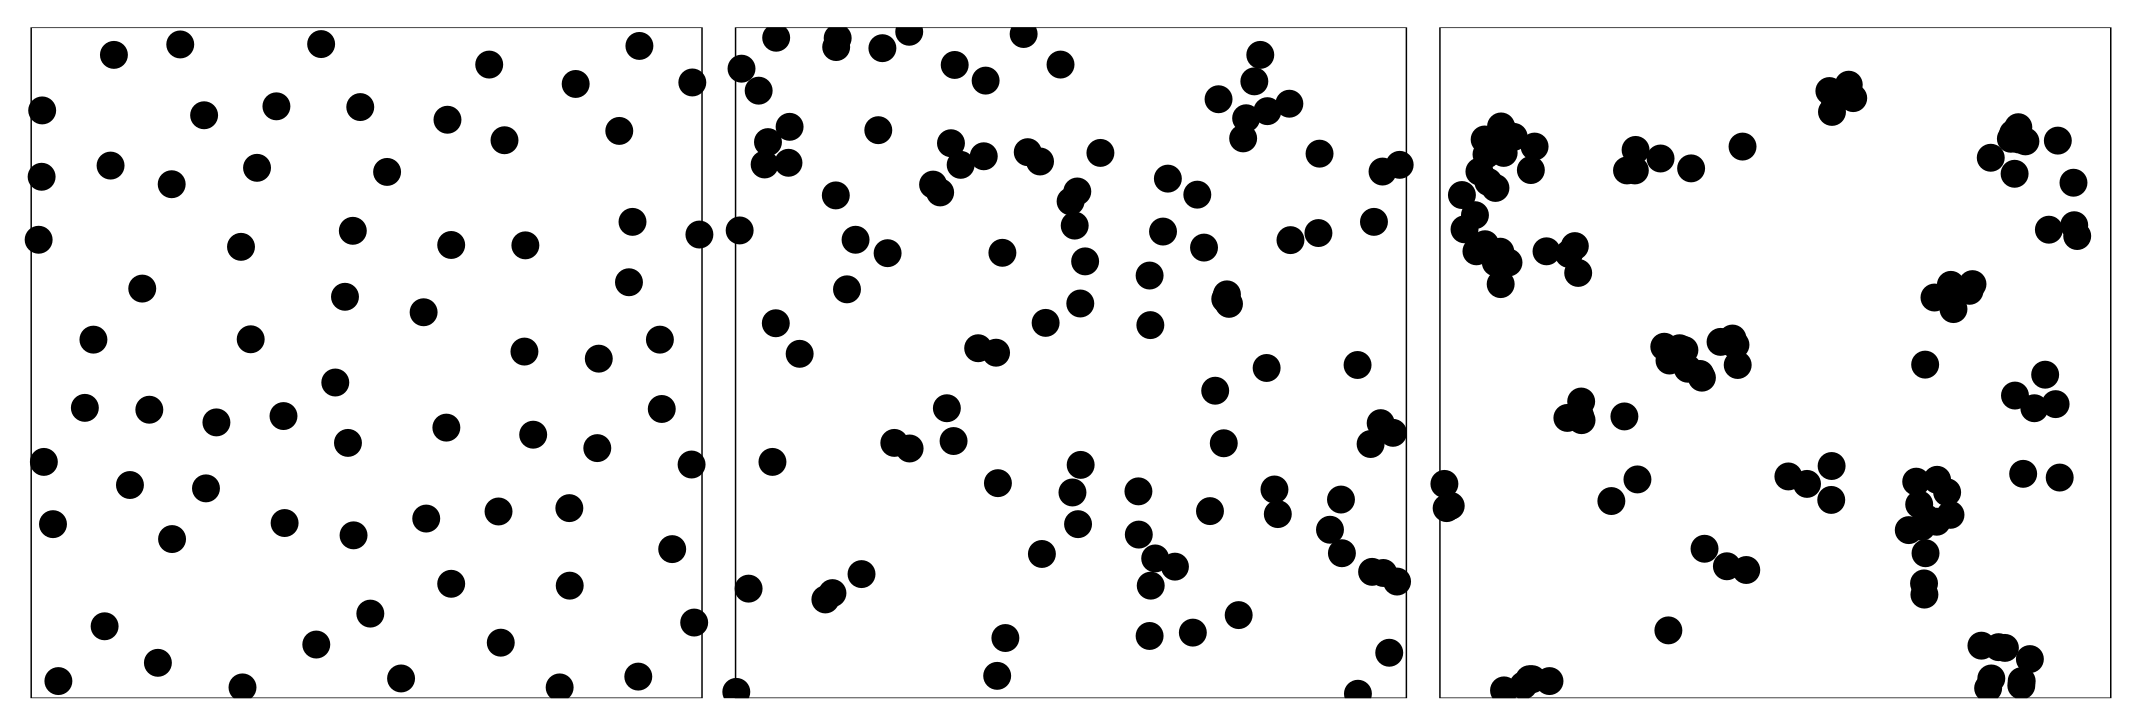
\includegraphics{Figuras/Ejemplo-procesos.png}
\end{frame}

\begin{frame}{Autocorrelación}
\protect\hypertarget{autocorrelaciuxf3n-1}{}
Moran-\emph{I} \textgreater{} 1

\begin{center}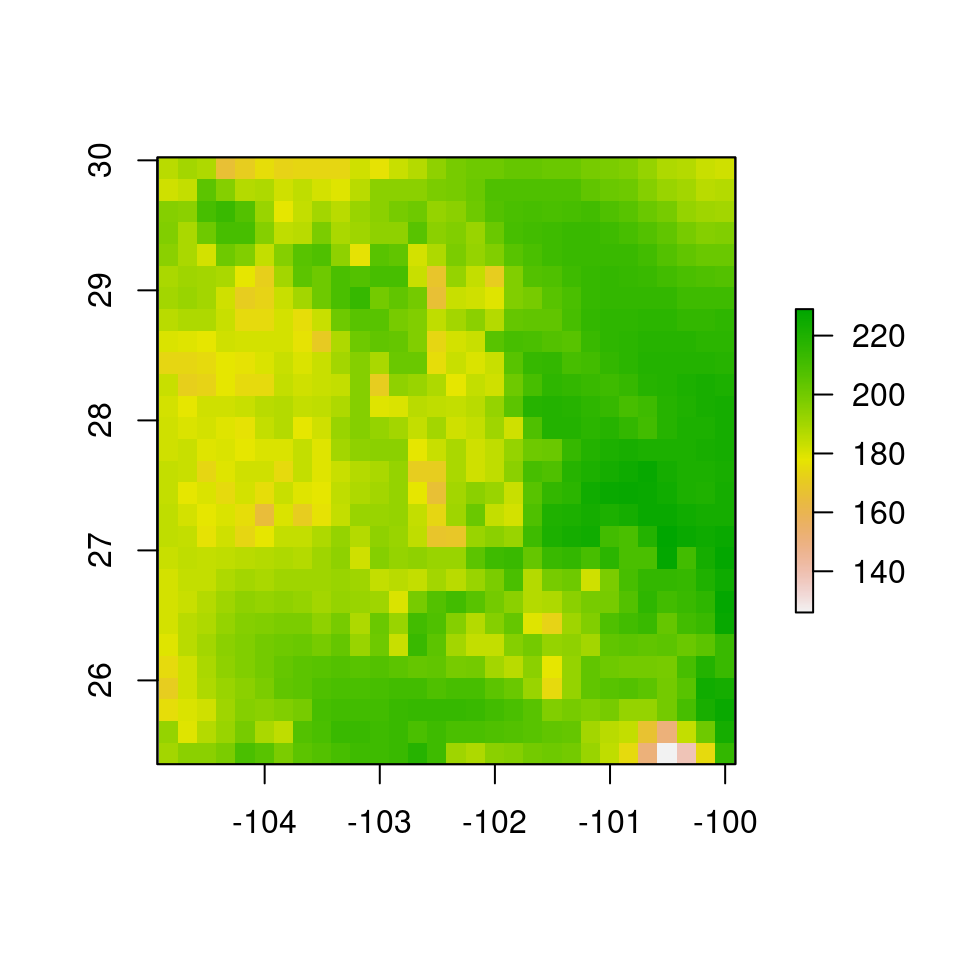
\includegraphics{Figuras/Moran-1-1} \end{center}
\end{frame}

\begin{frame}{Autocorrelación}
\protect\hypertarget{autocorrelaciuxf3n-2}{}
Moran-\emph{I} \(\approx\) 0

\begin{center}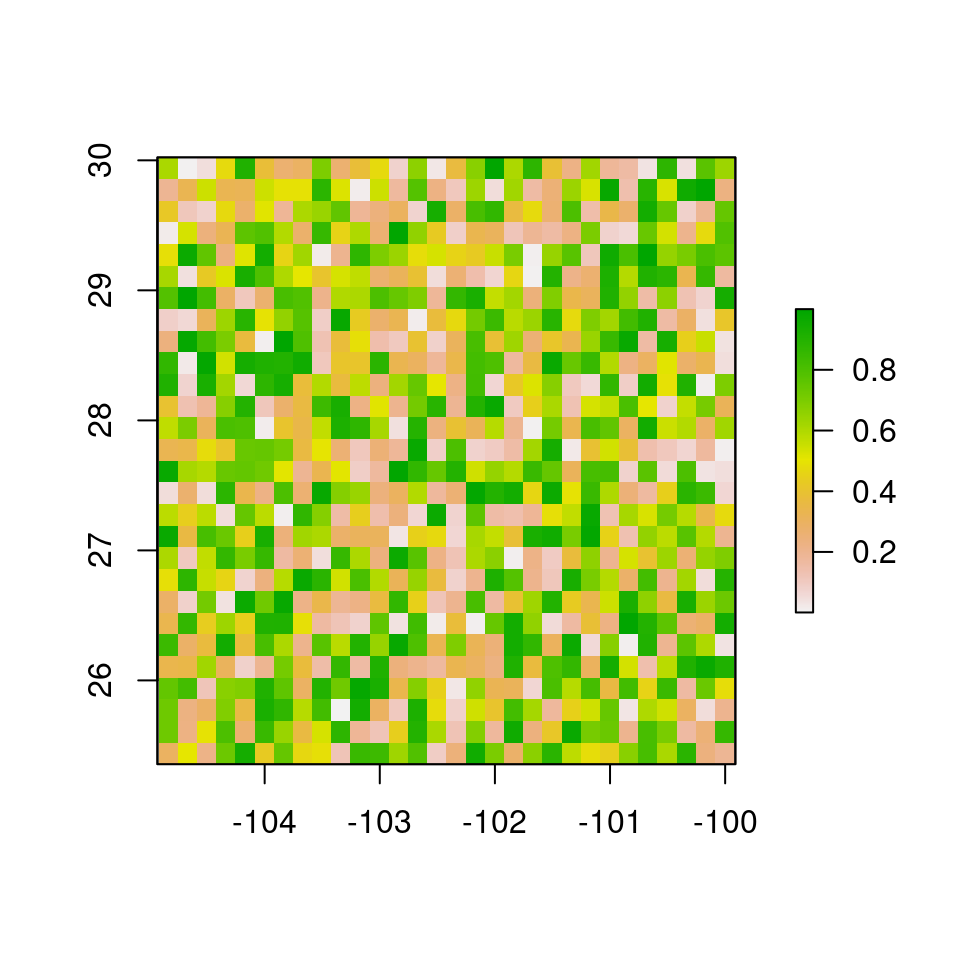
\includegraphics{Figuras/Moran-2-1} \end{center}
\end{frame}

\begin{frame}{Autocorrelación de PPs}
\protect\hypertarget{autocorrelaciuxf3n-de-pps}{}
Número de vecinos

\begin{center}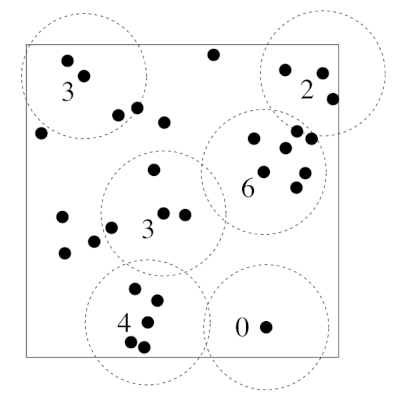
\includegraphics{Figuras/Cuenta-vecinos} \end{center}
\end{frame}

\begin{frame}{Autocorrelación de PPs}
\protect\hypertarget{autocorrelaciuxf3n-de-pps-1}{}
\begin{center}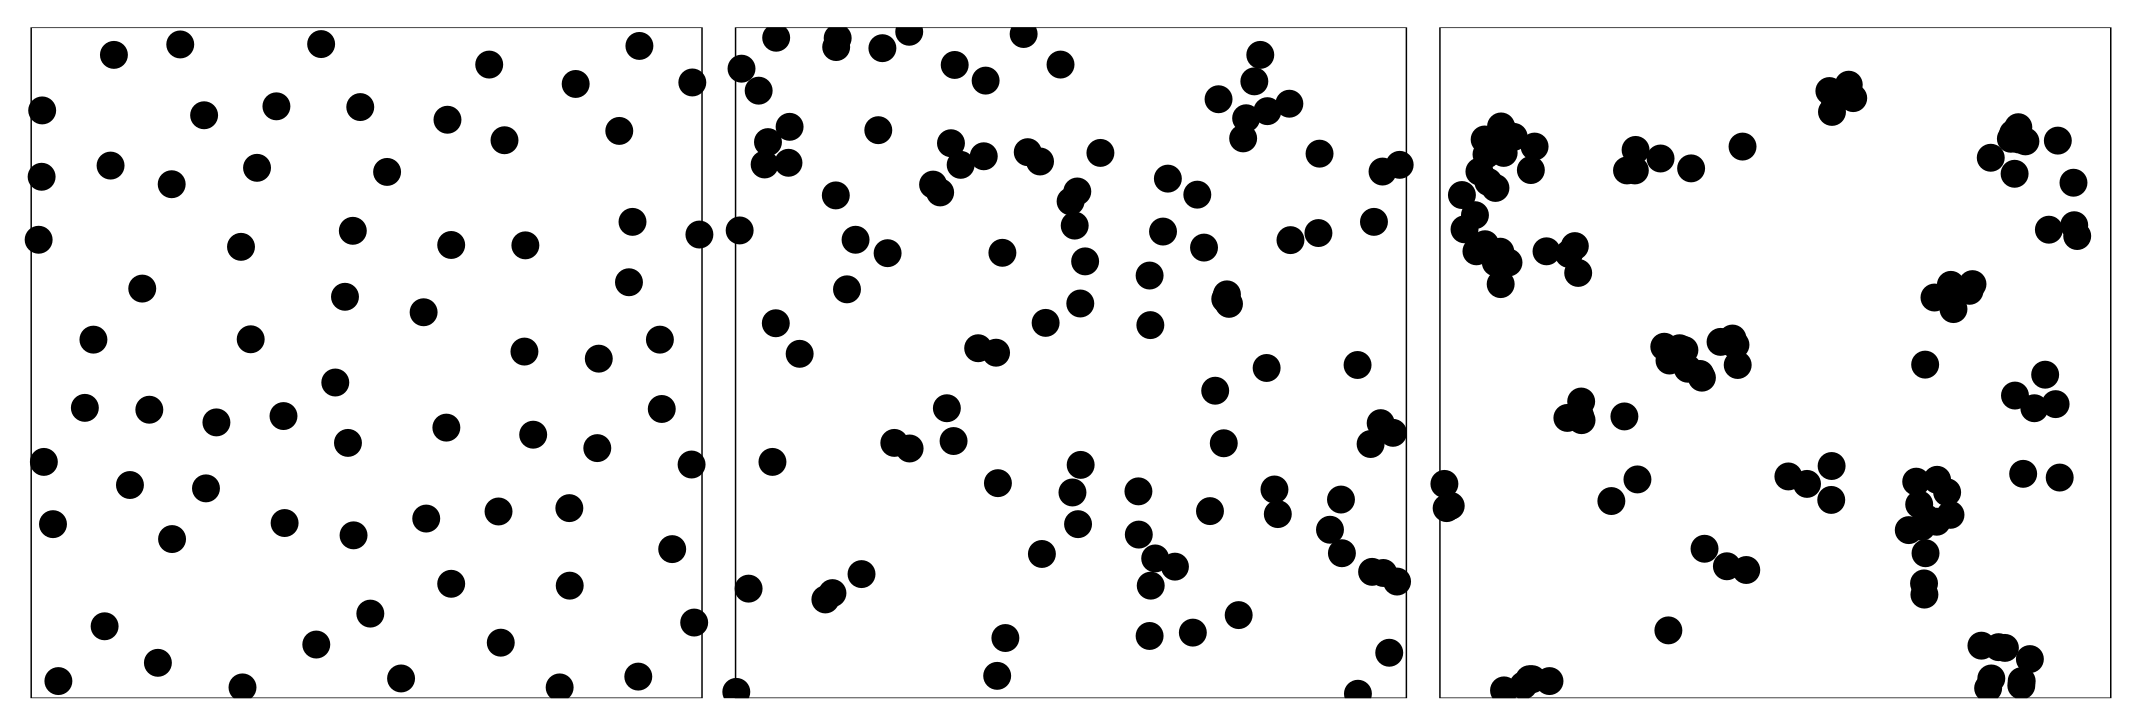
\includegraphics{Figuras/Ejemplo-procesos} \end{center}
\end{frame}

\begin{frame}{Autocorrelación de PPs}
\protect\hypertarget{autocorrelaciuxf3n-de-pps-2}{}
\begin{center}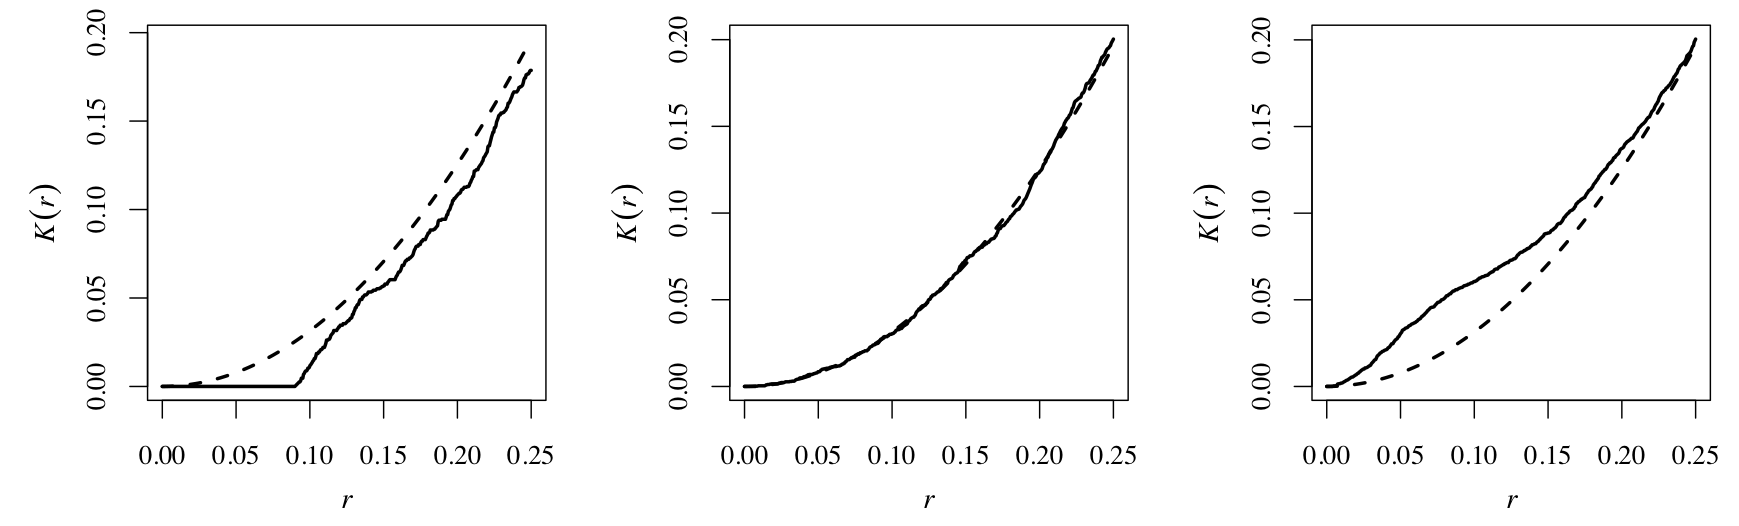
\includegraphics{Figuras/K-Ripley} \end{center}
\end{frame}

\begin{frame}{Autocorrelación de PPs}
\protect\hypertarget{autocorrelaciuxf3n-de-pps-3}{}
\begin{itemize}
\item
  Verificar, medir supuesto \(\rightarrow\) Proponer soluciones
\item
  Pruebas estadísticas

  \begin{itemize}
  \tightlist
  \item
    \emph{K} Ripley
  \item
    \emph{L} Besag
  \end{itemize}
\end{itemize}
\end{frame}

\hypertarget{causas-de-la-autocorrelaciuxf3n}{%
\section{Causas de la
autocorrelación}\label{causas-de-la-autocorrelaciuxf3n}}

\begin{frame}{Autocorrelación - causas}
\protect\hypertarget{autocorrelaciuxf3n---causas}{}
Tú

\begin{center}
\includegraphics{Figuras/Observ} \end{center}
\end{frame}

\begin{frame}{Autocorrelación - causas}
\protect\hypertarget{autocorrelaciuxf3n---causas-1}{}
Los bichos

\begin{center}
\includegraphics{Figuras/Bicho} \end{center}
\end{frame}

\begin{frame}{Autocorrelación - corrección}
\protect\hypertarget{autocorrelaciuxf3n---correcciuxf3n}{}
\begin{itemize}
\tightlist
\item
  Combinar geoestadística con regresión:
\end{itemize}

\[ \log \lambda(u) = \alpha + \beta_1 x_1 + \dots + \gamma(s) + \varepsilon \]
- \(x_i\) son las covariables ambientales (afectan media de \(\lambda\))

\begin{itemize}
\tightlist
\item
  \(\gamma\) es el efecto del espacio (Lo que \(x\) no explica)
\end{itemize}
\end{frame}

\begin{frame}[fragile]{Modelos para diferentes procesos de puntos}
\protect\hypertarget{modelos-para-diferentes-procesos-de-puntos}{}
\begin{itemize}
\item
  Puntos se repelen - Modelos de interacción
\item
  Puntos aleatorios - Modelos Poisson
\item
  Puntos moderadamente agregados - Modelos de interacción
\item
  Puntos altamente agregados - Modelos log-Cox Gaussianos, Clúster
\end{itemize}

\textbf{Todos implementados en \texttt{spatstat}}
\end{frame}

\end{document}
